\chapter{Background and Related Work}
\label{ch:background}
TODO: Not up to date, need rewrite of model names and some revision.

\section{Digital Journaling and Self-Reflection}

Digital journaling platforms have grown as tools for emotional awareness and habit tracking. Mood trackers, guided journaling apps, and reflective writing assistants help users notice patterns in their thoughts and behaviour. Prior research shows that structured journaling can improve emotional regulation and self-awareness \cite{Sivaram2022HealthyMe}.

Recent work has explored AI-assisted journaling, where NLP extracts insights from user text \cite{10351450}. These systems show that automated analysis can support personal reflection, but most rely on cloud-based processing, which raises privacy concerns.

\section{Natural Language Processing in Personal Well-Being}

NLP techniques have been widely applied to sentiment analysis, emotion detection, and mental health monitoring. Transformer-based models have become the dominant approach due to their contextual understanding. However, full-size models such as BERT are too computationally expensive for mobile deployment. Lightweight variants such as DistilBERT \cite{sanh2019distilbert}, TinyBERT \cite{jiao2020tinybert}, and MobileBERT \cite{sun2020mobilebert} run on device while maintaining competitive accuracy, making them practical for applications where sensitive data should not leave the device.

\section{On-Device Machine Learning}

On-device machine learning has grown in relevance due to improvements in mobile NPUs and the need for private computation. Research on edge-based emotion detection \cite{Pandelea2021EmotionEdge} and optimised clustering for mobile processors \cite{awad2022improved} shows that meaningful analysis can run locally. Frameworks such as Core ML and TensorFlow Lite support deployment of compact models on smartphones, enabling inference without network connectivity.

\section{Clustering and Semantic Analysis}

Clustering algorithms group semantically similar text entries. Density-based methods such as DBSCAN \cite{ester1996density} suit small, irregular datasets like personal journals because they do not require specifying the number of clusters in advance and can mark individual entries as noise. Recent work combining transformer embeddings with clustering has produced solid results for topic discovery and personal data organisation, and these techniques are what GJournal uses to group microjournal entries into themes.

\section{Mobile Hardware for On-Device AI}

Modern smartphones can run NLP models locally due to advances in dedicated silicon. Specialised Neural Processing Units (NPUs) in current devices perform billions of operations per second, making compact transformer inference practical.

\subsection{Evolution of Mobile NPUs}

Early smartphones used CPUs and GPUs for machine learning workloads, which produced high latency and significant energy draw. Dedicated NPUs changed this. Modern chipsets from Apple (A-series) and Qualcomm (Snapdragon 8-series) include hardware optimised for matrix multiplication, low-precision arithmetic, and transformer inference \cite{apple2023neuralengine,qualcomm2023hexagon}.

Tables~\ref{tab:apple_npu} and~\ref{tab:qualcomm_npu} summarise NPU performance (measured in TOPS, tera operations per second) across recent chip generations. Apple's A17 Pro reaches 35 TOPS; Qualcomm's Snapdragon 8 Gen 3 reaches 45 TOPS. Estimated values are included where manufacturers did not publish official figures.

\begin{table}[h]
\centering
\caption{NPU performance in Apple A-series chips (2019--2025).}
\label{tab:apple_npu}
\begin{tabular}{|c|l|l|c|}
\hline
\textbf{Year} & \textbf{Chip} & \textbf{Device} & \textbf{TOPS} \\
\hline
2019 & A13 Bionic   & iPhone 11        & $\sim$6 (est.) \\
2020 & A14 Bionic   & iPhone 12        & 11 \\
2021 & A15 Bionic   & iPhone 13        & 15.8 \\
2022 & A16 Bionic   & iPhone 14 Pro    & 17 \\
2023 & A17 Pro      & iPhone 15 Pro    & 35 \\
2024 & A18 / A18 Pro & iPhone 16 series & 35 \\
2025 & A19 Pro      & iPhone 17 Pro    & $\sim$38 (est.) \\
\hline
\end{tabular}
\end{table}

\begin{table}[h]
\centering
\caption{NPU performance in Qualcomm Snapdragon flagship chips (2021--2025).}
\label{tab:qualcomm_npu}
\begin{tabular}{|c|l|l|c|}
\hline
\textbf{Year} & \textbf{Chip} & \textbf{Device} & \textbf{TOPS} \\
\hline
2021 & Snapdragon 888    & Galaxy S21 & 26 \\
2022 & Snapdragon 8 Gen 1 & Galaxy S22 & $\sim$32 (est.) \\
2023 & Snapdragon 8 Gen 2 & Galaxy S23 & $\sim$40 (est.) \\
2024 & Snapdragon 8 Gen 3 & Galaxy S24 & 45 \\
2025 & Snapdragon 8 Elite & Galaxy S25 & $\sim$65 (est.) \\
\hline
\end{tabular}
\end{table}

Figure~\ref{fig:npu_tops} shows the growth trend across both chip families. The increase over the past five years makes transformer-based NLP on a smartphone practical rather than aspirational.

\begin{figure}[h]
\centering
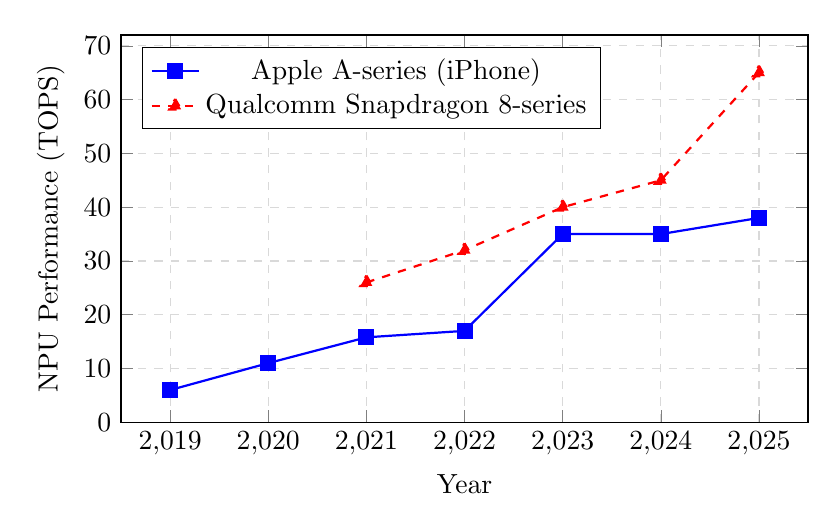
\begin{tikzpicture}
\begin{axis}[
    xlabel={Year},
    ylabel={NPU Performance (TOPS)},
    xmin=2018.5, xmax=2025.5,
    ymin=0, ymax=72,
    xtick={2019,2020,2021,2022,2023,2024,2025},
    ytick={0,10,20,30,40,50,60,70},
    legend pos=north west,
    grid=major,
    grid style={dashed,gray!30},
    width=0.85\textwidth,
    height=6.5cm,
    mark size=2.5pt,
]
\addplot[
    color=blue, mark=square*, thick
] coordinates {
    (2019,6)(2020,11)(2021,15.8)(2022,17)(2023,35)(2024,35)(2025,38)
};
\addlegendentry{Apple A-series (iPhone)}

\addplot[
    color=red, mark=triangle*, thick, dashed
] coordinates {
    (2021,26)(2022,32)(2023,40)(2024,45)(2025,65)
};
\addlegendentry{Qualcomm Snapdragon 8-series}
\end{axis}
\end{tikzpicture}
\caption{Growth of NPU performance (TOPS) across recent Apple and Qualcomm chipsets. Data from public specifications; estimated values marked in Tables~\ref{tab:apple_npu} and~\ref{tab:qualcomm_npu}.}
\label{fig:npu_tops}
\end{figure}

\subsection{Implications for On-Device NLP}

The compute available on modern NPUs is sufficient for real-time inference of lightweight transformer models such as MobileBERT, DistilBERT, and TinyBERT. These models have a small memory footprint, run at low latency, and support 8-bit and 16-bit quantisation, which means tasks like semantic embedding, emotion detection, and clustering can run entirely on the device.

\subsection{Privacy and Energy Considerations}

On-device processing means user data never leaves the device, which matters for journaling applications where entries often contain personal information. Modern NPUs also consume little power for inference, so background tasks like embedding generation and clustering have minimal battery impact.

\section{Summary}

Prior work shows that journaling supports self-reflection, that lightweight transformer models achieve competitive NLP quality on mobile hardware, and that DBSCAN-based clustering can group short personal texts into coherent themes. These three factors together make a privacy-preserving, on-device journaling system feasible with current smartphones.
